\documentclass{beamer}
\mode<presentation>
\usepackage{amsmath}
\usepackage{amssymb}
%\usepackage{advdate}
\usepackage{adjustbox}
\usepackage{subcaption}
\usepackage{enumitem}
\usepackage{multicol}
\usepackage{mathtools}
\usepackage{listings}
\usepackage{float}
\usepackage{graphicx}
\usepackage{url}
\def\UrlBreaks{\do\/\do-}
\usetheme{Boadilla}
\usecolortheme{lily}
\setbeamertemplate{footline}
{
  \leavevmode%
  \hbox{%
  \begin{beamercolorbox}[wd=\paperwidth,ht=2.25ex,dp=1ex,right]{author in head/foot}%
    \insertframenumber{} / \inserttotalframenumber\hspace*{2ex} 
  \end{beamercolorbox}}%
  \vskip0pt%
}
\setbeamertemplate{navigation symbols}{}

\providecommand{\nCr}[2]{\,^{#1}C_{#2}} % nCr
\providecommand{\nPr}[2]{\,^{#1}P_{#2}} % nPr
\providecommand{\mbf}{\mathbf}
\providecommand{\pr}[1]{\ensuremath{\Pr\left(#1\right)}}
\providecommand{\qfunc}[1]{\ensuremath{Q\left(#1\right)}}
\providecommand{\sbrak}[1]{\ensuremath{{}\left[#1\right]}}
\providecommand{\lsbrak}[1]{\ensuremath{{}\left[#1\right.}}
\providecommand{\rsbrak}[1]{\ensuremath{{}\left.#1\right]}}
\providecommand{\brak}[1]{\ensuremath{\left(#1\right)}}
\providecommand{\lbrak}[1]{\ensuremath{\left(#1\right.}}
\providecommand{\rbrak}[1]{\ensuremath{\left.#1\right)}}
\providecommand{\cbrak}[1]{\ensuremath{\left\{#1\right\}}}
\providecommand{\lcbrak}[1]{\ensuremath{\left\{#1\right.}}
\providecommand{\rcbrak}[1]{\ensuremath{\left.#1\right\}}}
\theoremstyle{remark}
\newtheorem{rem}{Remark}
\newcommand{\sgn}{\mathop{\mathrm{sgn}}}
\providecommand{\abs}[1]{\left\vert#1\right\vert}
\providecommand{\res}[1]{\Res\displaylimits_{#1}} 
\providecommand{\norm}[1]{\lVert#1\rVert}
\providecommand{\mtx}[1]{\mathbf{#1}}
\providecommand{\mean}[1]{E\left[ #1 \right]}
\providecommand{\fourier}{\overset{\mathcal{F}}{ \rightleftharpoons}}
%\providecommand{\hilbert}{\overset{\mathcal{H}}{ \rightleftharpoons}}
\providecommand{\system}{\overset{\mathcal{H}}{ \longleftrightarrow}}
	%\newcommand{\solution}[2]{\textbf{Solution:}{#1}}
%\newcommand{\solution}{\noindent \textbf{Solution: }}
\providecommand{\dec}[2]{\ensuremath{\overset{#1}{\underset{#2}{\gtrless}}}}
\newcommand{\myvec}[1]{\ensuremath{\begin{pmatrix}#1\end{pmatrix}}}
\let\vec\mathbf

\lstset{
language=C,
frame=single, 
breaklines=true,
columns=fullflexible
}

\numberwithin{equation}{section}

\title{Presentation - Matgeo}
\author{Aryansingh Sonaye \\
AI25BTECH11032 \\
EE1030 - Matrix Theory}

\date{\today} 
\begin{document}

\begin{frame}
\titlepage
\end{frame}

\section{Problem}
\begin{frame}
\frametitle{Problem Statement}
\textbf{Problem 5.3.26}
For what value of $k$, does the system of linear equations
\begin{align}
2x + 3y = 7, \qquad (k-1)x + (k+2)y = 3k
\end{align}
have an infinite number of solutions?

\end{frame}

\section{Solution}
\subsection{Description of Variables used}
\begin{frame}
\frametitle{Description of Variables used}
\begin{table}[H]
\centering
\begin{tabular}{|c|c|c|}
\hline
\textbf{Symbol} & \textbf{Description} & \textbf{Value/Expression} \\
\hline
$x,y$ & Unknown variables & Real numbers \\
$k$ & Parameter in system & To be determined \\
$\vec{x}$ & Unknown vector & $\myvec{x \\ y}$ \\
$A$ & Coefficient matrix & $\myvec{2 & 3 \\ k-1 & k+2}$ \\
$\vec{b}$ & RHS vector & $\myvec{7 \\ 3k}$ \\
$[A|b]$ & Augmented matrix & $\myvec{2 & 3 & 7 \\ k-1 & k+2 & 3k}$ \\
\hline
\end{tabular}
\caption{}
\label{}
\end{table}


\end{frame}

\subsection{Theoretical Solution }
\begin{frame}
\frametitle{Theoretical Solution}
\begin{align}
\myvec{2 & 3 \\ k-1 & k+2}\vec{x} &= \myvec{7 \\ 3k}, \quad 
\text{where } \vec{x} = \myvec{x \\ y}.
\end{align}

\begin{align}
\text{The augmented matrix is } 
\myvec{2 & 3 & 7 \\ k-1 & k+2 & 3k}.
\end{align}

\begin{align}
R_2 &\to R_2 - \tfrac{k-1}{2}R_1 \\[6pt]
\myvec{2 & 3 & 7 \\ k-1 & k+2 & 3k}
&\to 
\myvec{2 & 3 & 7 \\ 0 & (k+2) - \tfrac{3}{2}(k-1) & 3k - \tfrac{7}{2}(k-1)}.
\end{align}

\end{frame}

\begin{frame}
\frametitle{Theoretical Solution}
\begin{align}
&= \myvec{2 & 3 & 7 \\ 0 & \tfrac{-k+7}{2} & \tfrac{-k+7}{2}}.
\end{align}

\begin{align}
\text{For infinite solutions: } 
\operatorname{rank}(A) &= \operatorname{rank}([A|b]) < 2.
\end{align}

\begin{align}
\tfrac{-k+7}{2} &= 0 \quad \Longrightarrow \quad k=7.
\end{align}

\begin{align}
\text{When } k=7,\quad
\myvec{2 & 3 & 7 \\ 0 & 0 & 0},
\end{align}

\begin{align}
\operatorname{rank}(A) &= \operatorname{rank}([A|b])=1 < 2.
\end{align}

\end{frame}

\begin{frame}
\frametitle{Theoretical Solution}
\begin{align}
\therefore \quad \text{The system has infinitely many solutions when } 
\boxed{k=7}.
\end{align}


\end{frame}







\subsection{Plot}
\begin{frame}
    \frametitle{Plot}
\begin{figure}[H]
   \centering
   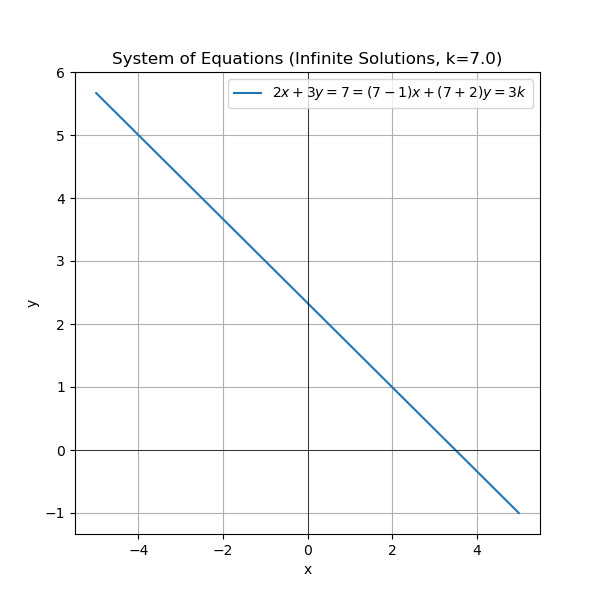
\includegraphics[width=0.7\columnwidth]{figs/infsols.png}
   \caption{}
   \label{}
   \end{figure}
\end{frame}

\begin{frame}[fragile]
    \frametitle{Code - C}
    \begin{lstlisting}
#include <stdio.h>

// Perform one step of row reduction on a 2x3 augmented matrix
void row_reduce(double A[2][3]) {
    if (A[0][0] != 0) {
        double factor = A[1][0] / A[0][0];
        for (int j = 0; j < 3; j++) {
            A[1][j] = A[1][j] - factor * A[0][j];
        }
    }
}

    \end{lstlisting}
    \end{frame}

\begin{frame}[fragile]
    \frametitle{Code - Python(with shared C code)}
    The code to obtain the required plot is
    \begin{lstlisting}
import ctypes
import numpy as np
import matplotlib.pyplot as plt
import sympy as sp

# Load the C shared library
lib = ctypes.CDLL("./row_reduction.so")
lib.row_reduce.argtypes = [
    np.ctypeslib.ndpointer(dtype=np.float64, ndim=2, flags="C_CONTIGUOUS")
]

def row_reduce(matrix):
    A = np.array(matrix, dtype=np.float64, order='C')
    lib.row_reduce(A)
    return A


\end{lstlisting}
\end{frame}
\begin{frame}[fragile]
\frametitle{Code - Python(with shared C code)}
\begin{lstlisting}
# Step 1: Solve for k using SymPy
k = sp.symbols('k')

# Row reduction condition: (-k+7)/2 = 0
expr = (-k + 7) / 2
solution = sp.solve(sp.Eq(expr, 0), k)
k_val = float(solution[0])   # numeric value for plotting

print(f"Calculated k = {k_val}")

# Step 2: Build augmented matrix with that k
A = np.array([
    [2, 3, 7],
    [k_val-1, k_val+2, 3*k_val]
], dtype=np.float64)


\end{lstlisting}
\end{frame}

\begin{frame}[fragile]
\frametitle{Code - Python(with shared C code)}
\begin{lstlisting}
print("\nOriginal Augmented Matrix:")
print(A)

# Step 3: Row reduction via C
reduced = row_reduce(A.copy())
print("\nRow Reduced Matrix:")
print(reduced)

# Step 4: Plot only the single line
x_vals = np.linspace(-5, 5, 400)

# General second equation: (k-1)x+(k+2)y=3k or y = (3k-(k-1)x)/(k+2)
y = (3*k_val - (k_val-1)*x_vals) / (k_val+2)



\end{lstlisting}
\end{frame}

\begin{frame}[fragile]
\frametitle{Code - Python(with shared C code)}
\begin{lstlisting}
plt.figure(figsize=(6,6))
plt.plot(x_vals, y, label=rf"$2x+3y=7 = ({int(k_val)}-1)x+({int(k_val)}+2)y=3k$")
plt.xlabel("x")
plt.ylabel("y")
plt.axhline(0, color='black', linewidth=0.5)
plt.axvline(0, color='black', linewidth=0.5)
plt.legend()
plt.grid(True)
plt.title(f"System of Equations (Infinite Solutions, k={k_val})")
plt.savefig("infsols.png")
plt.show()


\end{lstlisting}
\end{frame}


\begin{frame}[fragile]
\frametitle{Code - Python only}
\begin{lstlisting}
import numpy as np
import matplotlib.pyplot as plt
import sympy as sp

# Step 1: Solve for k using SymPy
k = sp.symbols('k')
expr = (-k + 7) / 2   # from row reduction condition
solution = sp.solve(sp.Eq(expr, 0), k)
k_val = float(solution[0])
print(f"Calculated k = {k_val}")

# Step 2: Build augmented matrix with NumPy
def augmented_matrix(k):
    return np.array([
        [2, 3, 7],
        [k-1, k+2, 3*k]
    ], dtype=float)



\end{lstlisting}
\end{frame}

\begin{frame}[fragile]
\frametitle{Code - Python only}
\begin{lstlisting}
A = augmented_matrix(k_val)
print("\nOriginal Augmented Matrix:")
print(A)

# Step 3: Row reduction in NumPy
def row_reduce(A):
    A = A.astype(float).copy()
    if A[0,0] != 0:
        factor = A[1,0] / A[0,0]
        A[1,:] = A[1,:] - factor * A[0,:]
    return A

R = row_reduce(A)
print("\nRow Reduced Matrix:")
print(R)



\end{lstlisting}
\end{frame}

\begin{frame}[fragile]
\frametitle{Code - Python only}
\begin{lstlisting}
# Step 4: Plot the single line
x_vals = np.linspace(-5, 5, 400)
# From (k-1)x+(k+2)y=3k or y = (3k-(k-1)x)/(k+2)
y_vals = (3*k_val - (k_val-1)*x_vals) / (k_val+2)

plt.figure(figsize=(6,6))
plt.plot(x_vals, y_vals, label=rf"$2x+3y=7 = ({int(k_val)}-1)x+({int(k_val)}+2)y=3k$")
plt.xlabel("x")
plt.ylabel("y")
plt.axhline(0, color='black', linewidth=0.5)
plt.axvline(0, color='black', linewidth=0.5)
plt.legend()
plt.grid(True)
plt.title(f"System of Equations (Infinite Solutions, k={k_val})")
plt.savefig("pyinfsols.png")
plt.show()


\end{lstlisting}
\end{frame}

\end{document}
